\documentclass[12pt]{article}
\usepackage[pdfborder={0 0 0.5 [3 2]}, plainpages=false]{hyperref}%
\usepackage[left=1in,right=1in,top=1in,bottom=1in]{geometry}%
\usepackage[shortalphabetic]{amsrefs}%
\usepackage{amsmath}
\usepackage{enumerate}
% \usepackage{enumitem}
\usepackage{amssymb}                
\usepackage{amsmath}                
\usepackage{amsfonts}
\usepackage{amsthm}
\usepackage{bbm}
\usepackage[table,xcdraw]{xcolor}
\usepackage{tikz}
\usepackage{float}
\usepackage{booktabs}
\usepackage{svg}
\usepackage{mathtools}
\usepackage{cool}
\usepackage{url}
\usepackage{graphicx,epsfig}
\usepackage{makecell}
\usepackage{array}

\usepackage[capitalize,nameinlink]{cleveref}
% Per SIAM Style Manual, "section" should be lowercase
\crefname{section}{section}{sections}
\crefname{subsection}{subsection}{subsections}
\Crefname{section}{Section}{Sections}
\Crefname{subsection}{Subsection}{Subsections}

% Per SIAM Style Manual, "Figure" should be spelled out in references
\Crefname{figure}{Figure}{Figures}

% Per SIAM Style Manual, don't say equation in front on an equation.
\crefformat{equation}{\textup{#2(#1)#3}}
\crefrangeformat{equation}{\textup{#3(#1)#4--#5(#2)#6}}
\crefmultiformat{equation}{\textup{#2(#1)#3}}{ and \textup{#2(#1)#3}}
{, \textup{#2(#1)#3}}{, and \textup{#2(#1)#3}}
\crefrangemultiformat{equation}{\textup{#3(#1)#4--#5(#2)#6}}%
{ and \textup{#3(#1)#4--#5(#2)#6}}{, \textup{#3(#1)#4--#5(#2)#6}}{, and \textup{#3(#1)#4--#5(#2)#6}}

% But spell it out at the beginning of a sentence.
\Crefformat{equation}{#2Equation~\textup{(#1)}#3}
\Crefrangeformat{equation}{Equations~\textup{#3(#1)#4--#5(#2)#6}}
\Crefmultiformat{equation}{Equations~\textup{#2(#1)#3}}{ and \textup{#2(#1)#3}}
{, \textup{#2(#1)#3}}{, and \textup{#2(#1)#3}}
\Crefrangemultiformat{equation}{Equations~\textup{#3(#1)#4--#5(#2)#6}}%
{ and \textup{#3(#1)#4--#5(#2)#6}}{, \textup{#3(#1)#4--#5(#2)#6}}{, and \textup{#3(#1)#4--#5(#2)#6}}

% Make number non-italic in any environment.
\crefdefaultlabelformat{#2\textup{#1}#3}

\def\noi{\noindent}
\def\T{{\mathbb T}}
\def\R{{\mathbb R}}
\def\N{{\mathbb N}}
\def\C{{\mathbb C}}
\def\Z{{\mathbb Z}}
\def\P{{\mathbb P}}
\def\E{{\mathbb E}}
\def\Q{\mathbb{Q}}
\def\ind{{\mathbb I}}

\DeclareMathOperator{\spn}{span}
\DeclareMathOperator{\ran}{range}
\DeclareMathOperator{\diag}{diag}


\graphicspath{ {images/} }

\newtheorem{lemma}{Lemma}
\newtheorem{theorem}{Theorem}
\newtheorem{corollary}{Corollary}
\newtheorem{definition}{Definition}
\newtheorem{proposition}{Proposition}
\newtheorem{hypothesis}{Hypothesis}

\newtheorem{notation}{Notation}

\begin{document}

Multi-core waveguides composed of $N$ twisted fibers arranged in a ring, propagation dynamics in setting of no gain/loss described by 
\begin{equation}\label{eq:twist1}
i \partial_z c_n = k \left(e^{-i\phi}c_{n+1} + e^{i\phi}c_{n-1}\right) + d |c_n|^2 c_n,
\end{equation}
which is \cite[(2.1)]{castro2016}. The degree of twisting is represented by $\phi$. As in DNLS, we are interested in standing wave solutions, which are bound states that can be written in the form
\begin{equation}\label{eq:ansatz1}
c_n = a_n e^{i (\omega z + \theta_n) },
\end{equation}
where $a_n \in \R$ and $\theta_n \in (-\pi/2, \pi/2]$. (Allowing $a_n$ to be negative lets us restrict $\theta_n$ in this way). Making this substitution, equation \cref{eq:twist1} becomes (after simplification)
\begin{equation}\label{eq:twisteq}
k\left( a_{n+1} e^{i((\theta_{n+1}-\theta_n)-\phi)} + a_{n-1} e^{-i((\theta_n - \theta_{n-1})-\phi)}\right) + \omega a_n + d a_n^3 = 0
\end{equation}
Note that the the exponential terms depend only on the phase differences between adjacent sites. Separating into real and imaginary parts, we have the $2n$ equations
\begin{equation}\label{eq:twisteqreal}
\begin{aligned}
k\left( a_{n+1} \cos(\theta_{n+1}-\theta_n-\phi) + a_{n-1} \cos(\theta_n - \theta_{n-1}-\phi)\right) + \omega a_n + d a_n^3 &= 0 \\\
a_{n+1} \sin(\theta_{n+1}-\theta_n-\phi) - a_{n-1} \sin(\theta_n - \theta_{n-1}-\phi) &= 0
\end{aligned}
\end{equation}
Due to the gauge invariance of \cref{eq:twist1}, we may without loss of generality take $\theta_1 = 0$. If $\phi = 0$ (no twist), we can take $\theta_n = 0$ for all $n$, which is the untwisted case with perioidic boundary conditions. Similarly, if we take $\phi = 2 \pi/N$ and $\theta_n = (n-1)\phi$ for $n = 1, \dots, N$, the ``twist'' terms in \cref{eq:twisteq} do not contribute, and the magnitudes $a_n$ are the same as in the untwisted case. The more interesting case is when $0 < \theta < 2 \pi/N$.

In the AC limit ($k = 0$), the sites are decoupled: each $a_n$ can take on any of the values 0, $\pm \sqrt{\omega}$, the phases $\theta_n$ can take on any value, and $\phi$ does not contribute. To construct solutions, we use AUTO for parameter continuation from the AC limit. For the an initial condition, we take $a = (1, 0, \dots, 0)$ (only one excited site) with $\theta_n = 0$ for all $n$ and $\phi = 0$. We first continue in the coupling parameter $k$, and then, for fixed $k$, we continue in the twist parameter $\phi$. In doing this, we find that the solutions have the following symmetry:
\begin{equation}
\begin{aligned}
a_k &= a_{N-k+2} && k = 2, \dots, M-1 \\
\theta_k &= -a_{N-k+2} && k = 2, \dots, M-1 
\end{aligned}
\end{equation}
where $M = (N/2)+1$ for $N$ even and $M = (N+1)/2$ for $N$ odd. In addition, for $N$ even, $\theta_M = 0$. 

For $N$ even, using these symmetries, as well as $\theta_0 = \theta_M = 0$, the system \cref{eq:twisteqreal} reduces to the system of equations
\begin{equation}\label{eq:twisteqeven}
\begin{aligned}
&2 k a_2 \cos(\theta_2 - \phi) + \omega a_1 + d a_1^3 = 0 \\
&k\left( a_3 \cos(\theta_3-\theta_2-\phi) + a_1 \cos(\theta_2-\phi)\right) + \omega a_2 + d a_2^3 = 0 \\
&a_3 \sin(\theta_3-\theta_2-\phi) - a_1 \sin(\theta_2-\phi) = 0 \\
&k\left( a_{n+1} \cos(\theta_{n+1}-\theta_n-\phi) + a_{n-1} \cos(\theta_n - \theta_{n-1}-\phi)\right) + \omega a_n + d a_n^3 = 0 && n = 3, \dots, M-2 \\
&a_{n+1} \sin(\theta_{n+1}-\theta_n-\phi) - a_{n-1} \sin(\theta_n - \theta_{n-1}-\phi) = 0 && n = 3, \dots, M-2 \\
&k\left( a_M \cos(-\theta_{M-1}-\phi) + a_{M-2} \cos(\theta_{M-1} - \theta_{M-2}-\phi)\right) + \omega a_{M-1} + d a_{M-1}^3 = 0 \\
&a_M \sin(-\theta_{M-1} -\phi) - a_{M-2} \sin(\theta_{M-1} - \theta_{M-2}-\phi) = 0 \\
&2 k a_{M-1} \cos(\theta_{M-1} + \phi) + \omega a_M + d a_M^3 = 0
\end{aligned}
\end{equation}

From the numerical parameter continuation, we see that when $\phi = \pi/N$, node $M$ (the nod) opposite the node with maximum excitation) has an amplitude of 0, i.e. is a dark node. If $a_M = 0$, then it follow from \cref{eq:twisteqeven} that $a_n = 0$ for all $n$ unless
\begin{equation}\label{eq:evendarknodecond}
\begin{aligned}
&\theta_{M-1} + \phi = \pi/2 \\
&\theta_{n} - \theta_{n-1} - \phi = 0 && n = 3, \dots, M-1 \\
&\theta_2 - \phi = 0
\end{aligned}
\end{equation}
from which it follows that $\phi = \pi/N$, which agrees with the numerical results. For this case, $a_M = 0$, $\theta_n = (n-1)\phi$, and \cref{eq:twisteqeven} reduces to the simpler system of equations
\begin{equation}\label{eq:twisteqevenhole}
\begin{aligned}
&2 k a_2 + \omega a_1 + d a_1^3 = 0 \\
&k\left( a_{n+1} + a_{n-1} \right) + \omega a_n + d a_n^3 = 0 && n = 2, \dots, M-2 \\
&k a_{M-2} + \omega a_{M-1} + d a_{M-1}^3 = 0 \\
\end{aligned}
\end{equation}
\cref{fig:evenhole6} shows this solution for $N=6$. This observation of a dark node for $N = 6$ when $\phi = \pi/6$ agrees with what was shown in \cite{castro2016}.

\begin{figure}[H]
\begin{center}
\begin{tabular}{c}
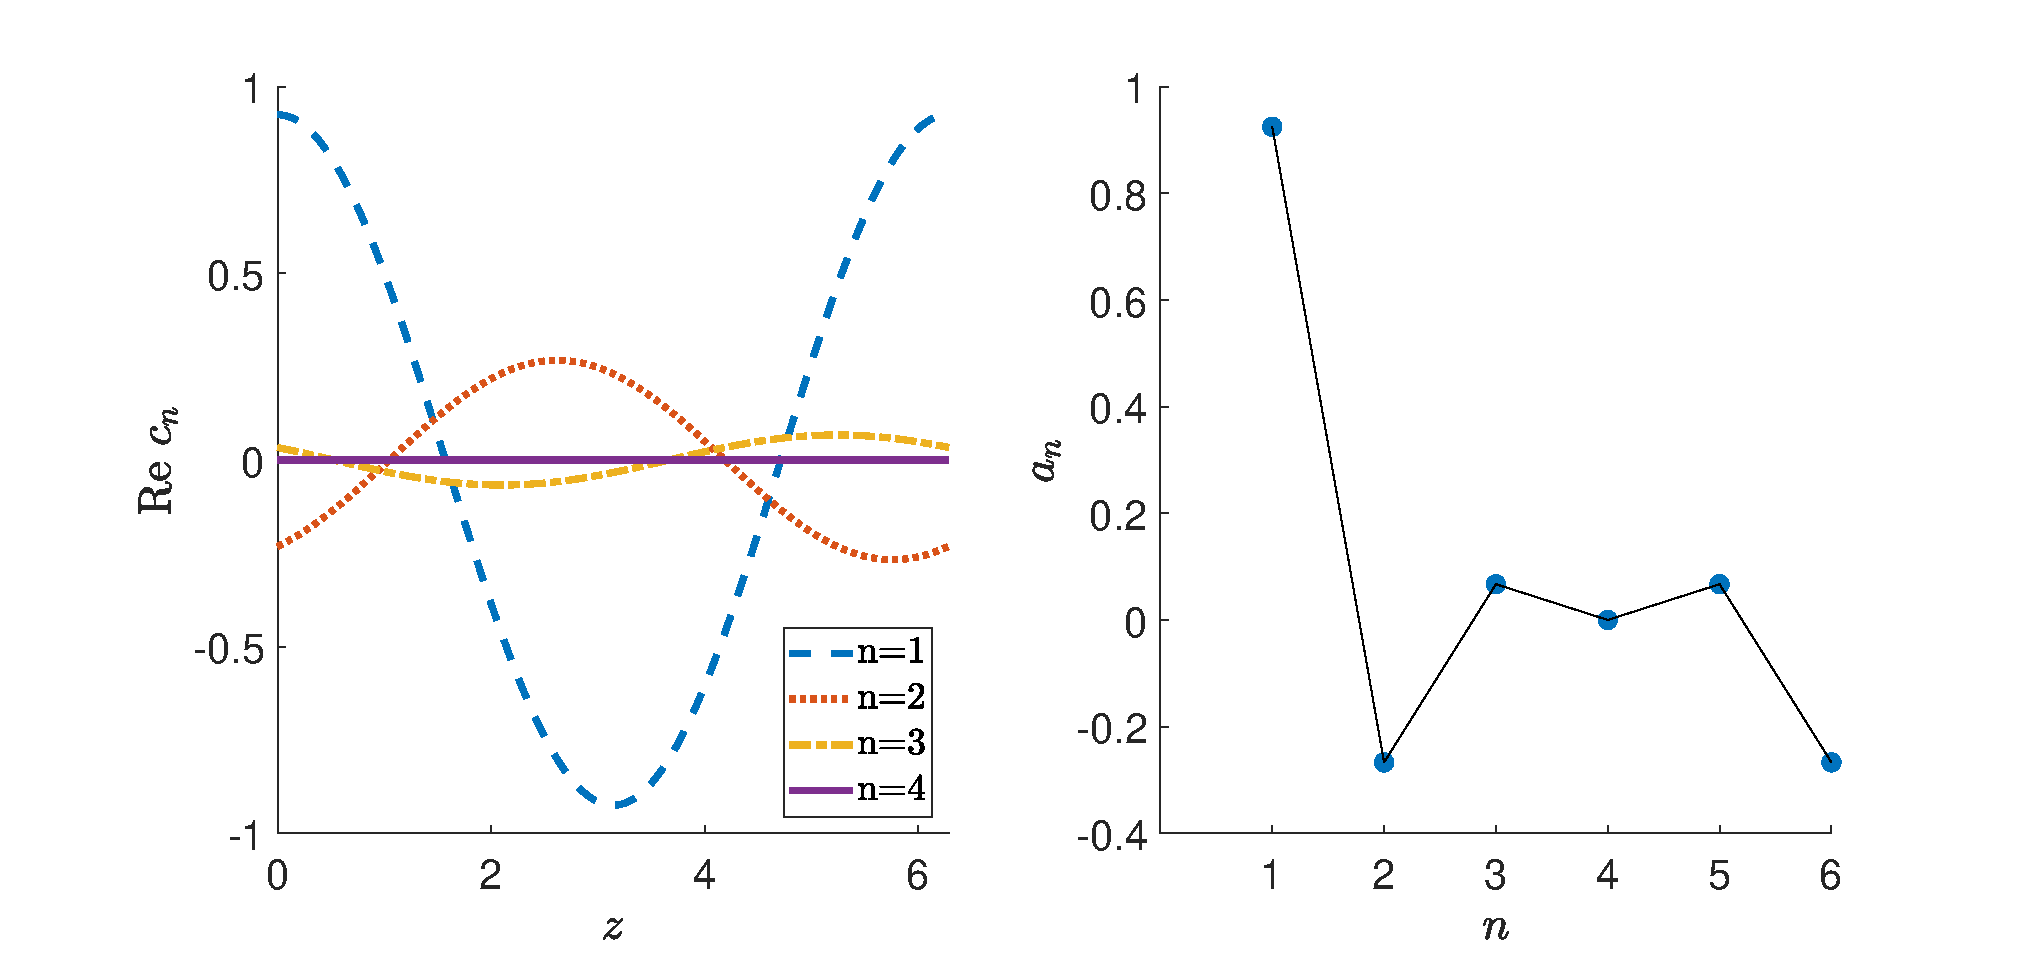
\includegraphics[width=15cm]{images/evenhole6.eps}
\end{tabular}
\end{center}
\caption{Standing wave solution for $N = 6$ and $\phi = \pi/6$. Left is real part of solution for each node, right is absolute value of solution at each node (this is constant in $t$). Node 1 has maximum amplitude, and node 4 is a dark node. $\omega = 1$, $k = 0.25$, $d=-1$.}
\label{fig:evenhole6}
\end{figure}

For $N$ odd, using the symmetries above, the system \cref{eq:twisteqreal} reduces to the system of equations
\begin{equation}\label{eq:twisteqeven}
\begin{aligned}
&2 k a_2 \cos(\theta_2 - \phi) + \omega a_1 + d a_1^3 = 0 \\
&k\left( a_3 \cos(\theta_3-\theta_2-\phi) + a_1 \cos(\theta_2-\phi)\right) + \omega a_2 + d a_2^3 = 0 \\
&a_3 \sin(\theta_3-\theta_2-\phi) - a_1 \sin(\theta_2-\phi) = 0 \\
&k\left( a_{n+1} \cos(\theta_{n+1}-\theta_n-\phi) + a_{n-1} \cos(\theta_n - \theta_{n-1}-\phi)\right) + \omega a_n + d a_n^3 = 0 && n = 3, \dots, M-1 \\
&a_{n+1} \sin(\theta_{n+1}-\theta_n-\phi) - a_{n-1} \sin(\theta_n - \theta_{n-1}-\phi) = 0 && n = 3, \dots, M-1 \\
&k ( a_M \cos(-2 \theta_M - \phi) + a_{M-1} \cos(\theta_M - \theta_{M-1} - \phi)) + \omega a_M + d a_M^3 = 0 \\
& a_M \sin(-2 \theta_M - \phi) - a_{M-1} \sin(\theta_M - \theta_{M-1} - \phi) = 0
\end{aligned}
\end{equation}
In this case, it follows from \cref{eq:twisteqeven} that if $a_M = 0$, then $a_n = 0$ for all $n$, thus for this symmetry, there are no solutions with a dark node if $N$ is odd. You might be able to get a dark node for $N$ odd if you start with two adjacent excited nodes in the AC limit.

For spectral stability and results of timestepping, all solutions generated this way (from AC limit with single excited node) are spectrally neutrally stable, for both $N$ even and $N$ odd. Spectrum is purely imaginary. In particular, this is true for the case with even $N$ and a dark node. Timestepping for a perturbation of this is shown in \cref{fig:oddhole7}.

\begin{figure}[H]
\begin{center}
\begin{tabular}{c}
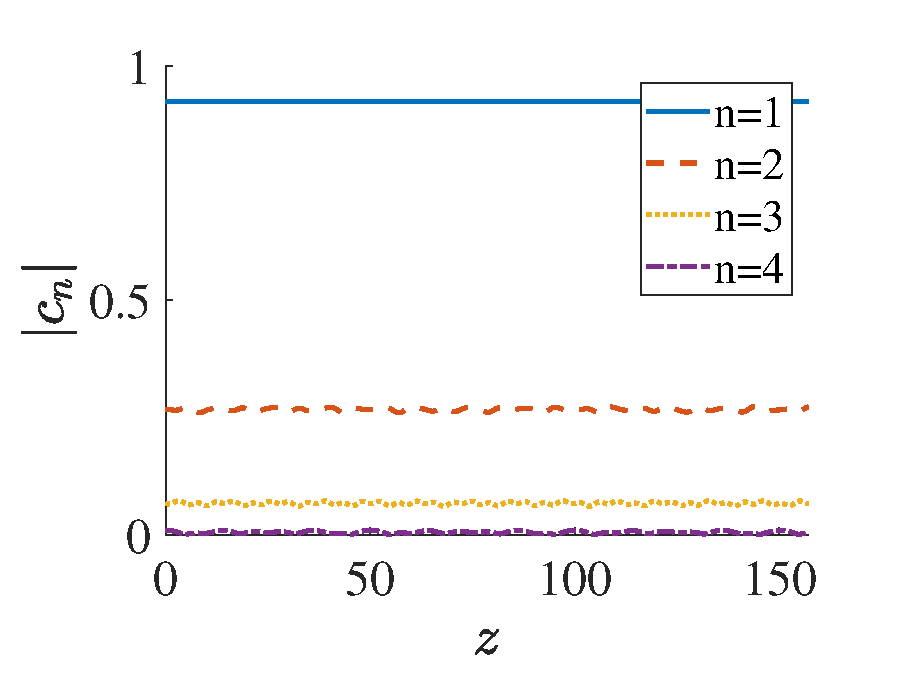
\includegraphics[width=10cm]{images/evenhole6perturbed.eps}
\end{tabular}
\end{center}
\caption{$|c_n|$ versus $t$. Solution with $N=6$ with dark node, perturbed by adding 0.01 to initial condition at dark node. RK4 for timestepping, $k=0.25$, $d=-1$.}
\label{fig:evenhole6perturbed}
\end{figure}


\bibliographystyle{amsplain}
\bibliography{twist.bib}


\end{document}